\begin{figure}[h]
	\centering
	\adjustbox{height=0.3\textheight}{
		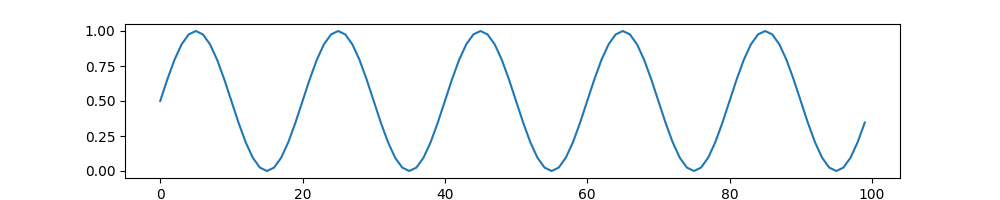
\includegraphics{img/methodology/signal.png}
	}
	\label{fig:methodology:signal}
	\caption[The example signal, with function $f(t)=\sin(\frac{15 \pi t}{500}) + \frac{t}{500}$.]{The example signal, with function $f(t)=\sin(\frac{15 \pi t}{500}) + \frac{t}{500}$. \change{The $t$ variable correspond to the time instant, while the $f(t)$ function gives the magnitude of the signal.}}
\end{figure}
